% !TEX root = ../thesis.tex

\chapter{Results}
\mbox{}\\
\mbox{}\\
\mbox{}\\
As described in the previous chapter, different strategies were elaborated for the reward function and the action selection algorithm. Training all possible combinations and then observing the end precision would be a viable way of finding the optimal combination of these. However, due to the training time of the algorithm, this would be very time intensive. I used the following techniques in order to find the best algorithms.
\section{Reward function selection}
As a reminder, if we view the problem as a decision tree, and the role of reinforcement learning to pick the best path at each node. The reward function can be viewed as the compass of the RL algorithm that should leading the algorithm to the end in such a way as to maximise the global goal.\\
I decided to measure the effectiveness of each reward function by observing if the direction it steered the algorithm to, was indeed correctly maximising this global goal. To achieve this, I would first train an algorithm with each of the different reward functions. Once this was done, I modified the Q-learning version of the algorithm so that during testing it would measure each of the different reward functions. As a reminder, the Q-learning algorithm was trained with the following reward function:
\begin{equation}
	r(s_t,a_t,s_{t+1}) = 3  \cdot n_s + 2 \cdot n_b + n_{hb} - \log_{10}(cyc)
\end{equation}
I would then run the Q-learning algorithm and each of the reward function algorithms measuring their reward during the execution. The decision of wether or not the reward function was correct was then made with the following rule:\\
If the reward of the deep Q-network algorithm was higher than the one of the Q-learning algorithm, but its overall precision was not higher. This would imply that the deep Q-network was correctly learning to maximise the reward, but that this reward was not maximising the overall performance of the algorithm and therefore that it was not a good reward.\\
As a reminder, the rewards tested are the following:
 
\begin{equation}
		r_{pr_1}(s_t,a_t,s_{t+1}) = 3  \cdot n_s + 2 \cdot n_b + n_{hb}
\end{equation}
\begin{equation}
		r_{pr_2}(s_t,a_t,s_{t+1}) = 3  \cdot n_s + 2 \cdot n_b + n_{hb} - \log_{10}(|n_b|)
\end{equation}
\begin{equation}
		r_{pr_3}(s_t,a_t,s_{t+1}) = 3  \cdot (n_{s_f} - n_{s_i}) + 2 \cdot (n_{b_f} - n_{b_i}) + (n_{hb_f} - n_{hb_i}) - \log_{10}(|n_b|)
\end{equation}

\begin{figure}[!h]
\minipage{0.32\textwidth}
  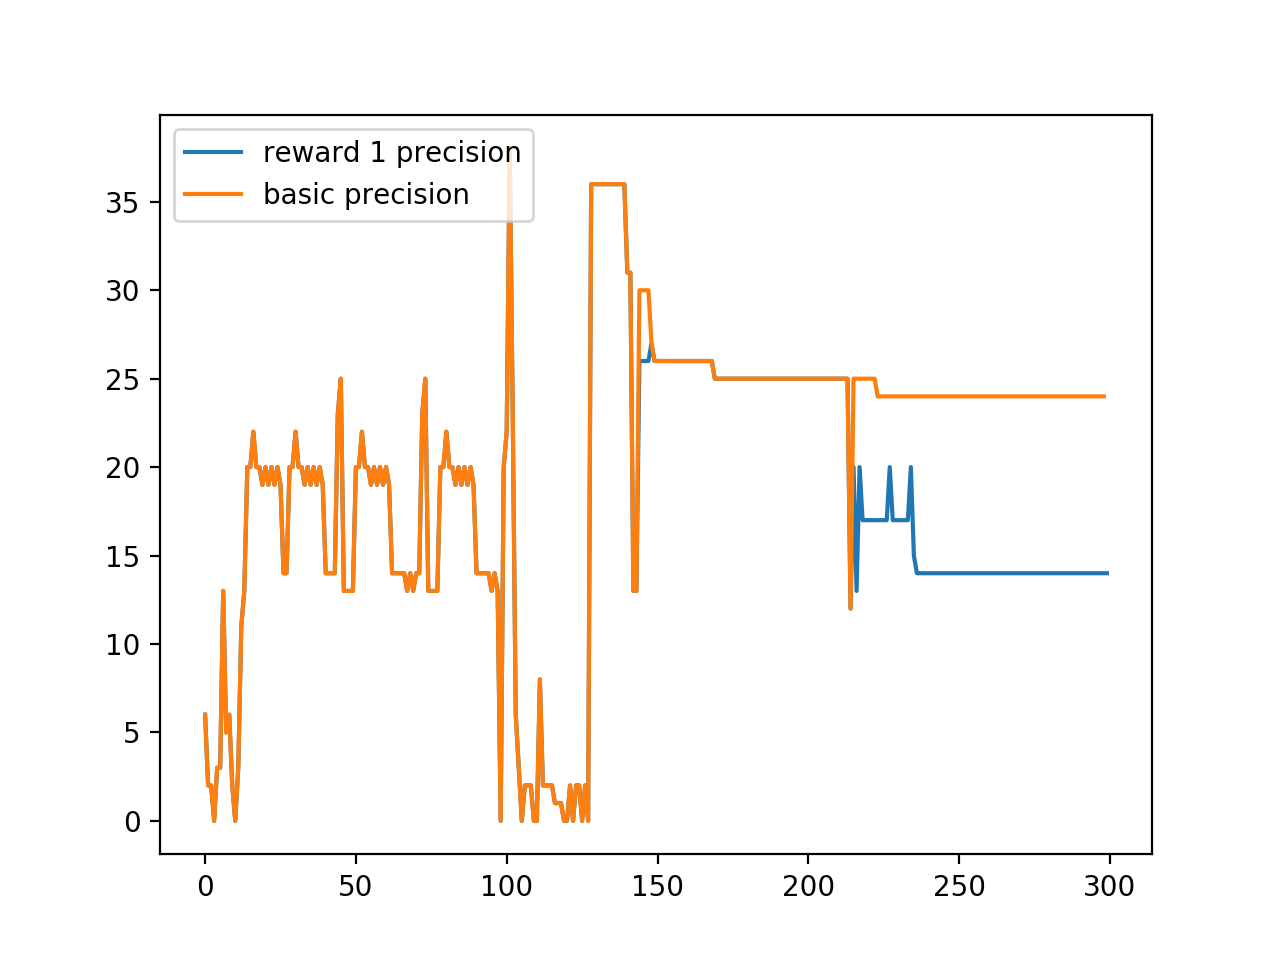
\includegraphics[width=7cm]{figures/r1}
  \caption{Reward one}\label{fig:r1}
\endminipage\hfill
\minipage{0.32\textwidth}
  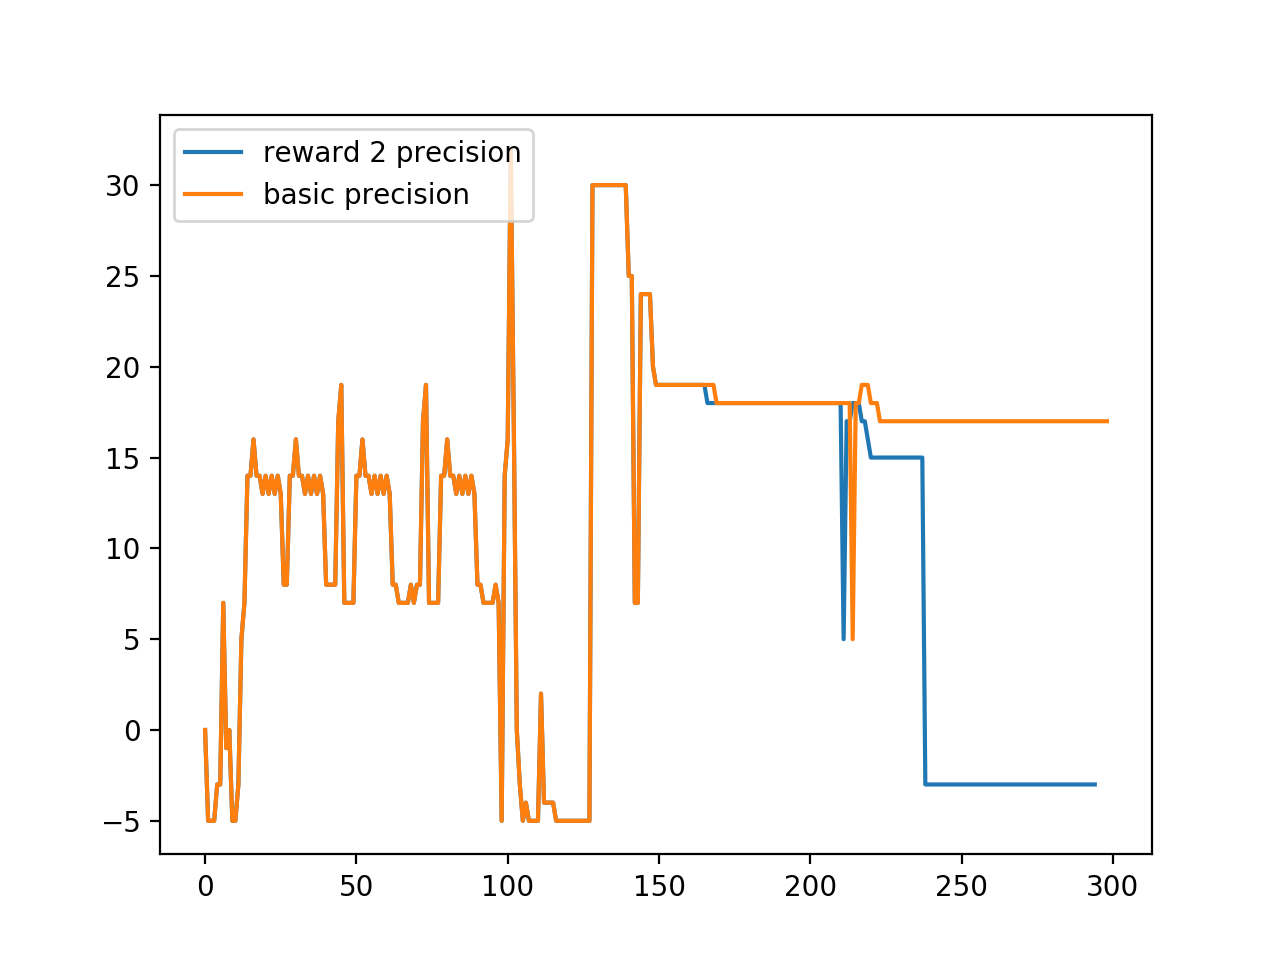
\includegraphics[width=7cm]{figures/r2}
  \caption{Reward two}\label{fig:r2}
\endminipage\hfill
\minipage{0.32\textwidth}%
  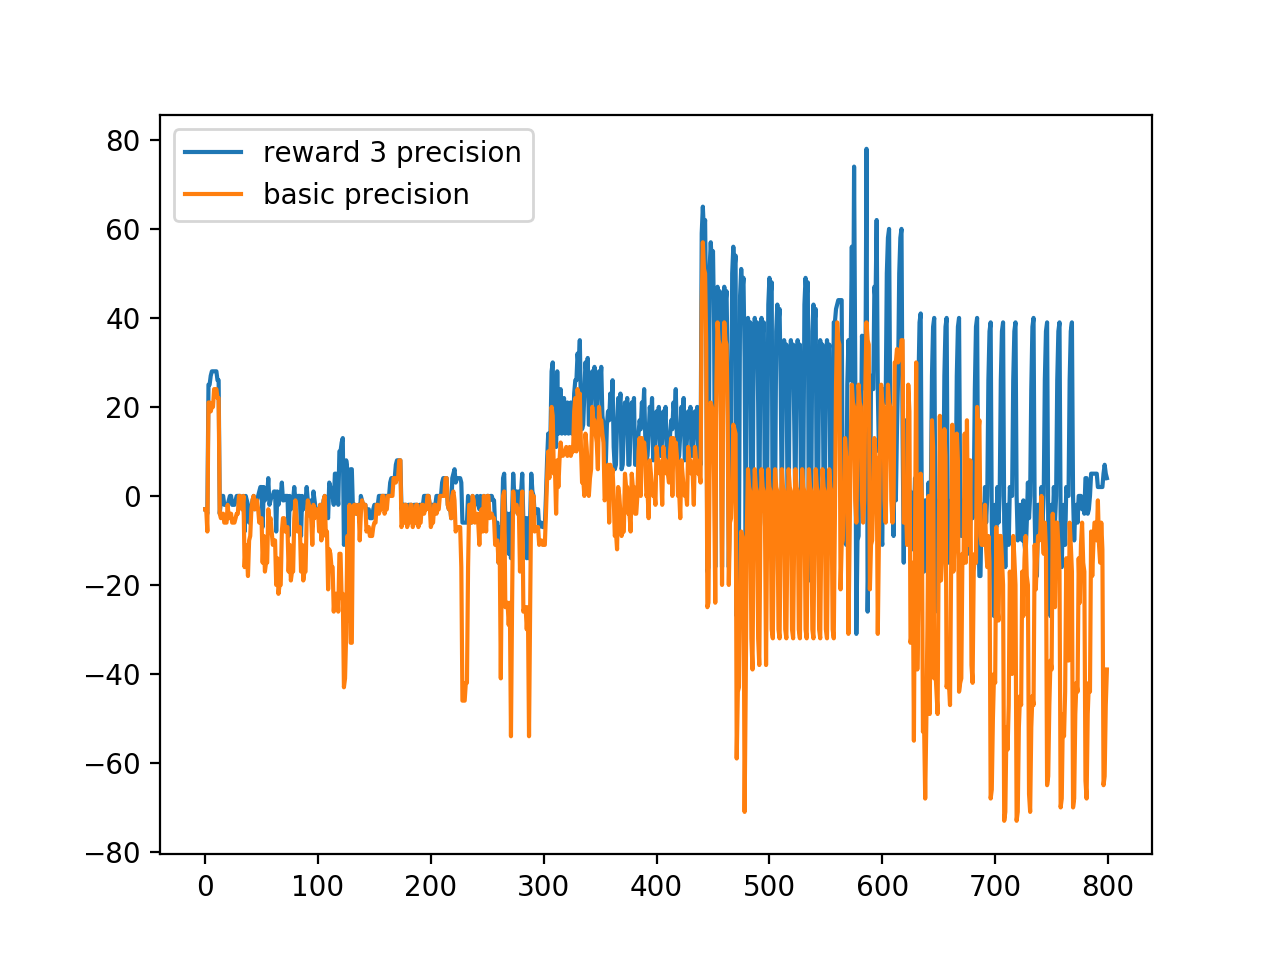
\includegraphics[width=7cm]{figures/r3}
  \caption{Reward three}\label{fig:r3}
\endminipage
\end{figure}
\mbox{}\\ \mbox{}\\

These are the graphs of the evolution of the precision reward according to the number of joins. The orange line represents the measured reward whilst running the Q-learning algorithm and the blue line the measured reward of the deep Q-network algorithm trained with this reward as well. The overall precision of the end polyhedra are the following: For Figure 5.1. 99\% for Q-learning and 96\% for DQN. For figure 5.2. 99\% for Q-learning and 94\% for DQN. For figure 5.3. 97\% for Q-learning and 90\% for DQN. Whilst these graphs behave as expected in the first two scenarios, that is that the reward is lower for the algorithm with lower end precision as well. In the last graph we can see something unexpected. Whilst the DQN algorithm has a higher reward throughout most of the execution of the program having an average of 9 versus -8 for the Q-learning algorithm. This tells us that whilst the DQN has learned a correct strategy for maximising the reward, this reward does not guide us to the overall goal of maximising the end precision and therefore reward three is not an optimal reward function. These experiments do not give us much information on the differences between reward one and two as they both behave as normally. This is to be expected as reward one and two are similar.\\
It is worth noting that whilst these experiments do give us some interesting information about the optimality of the different reward function, the results are heavily dependant of the benchmark we run them on and therefore the results cannot be fully trusted. However, with the information gathered by these experiments as well as some overall testing I decided to use the second reward function in further experiments.


\section{Action selection algorithm}
The second problem was selection the best action selection algorithm. In section 4.8., four different action selection algorithm were described. In order to select the best one of these four, I proceeded by training an algorithm using each of these four selection algorithms and then comparing the overall precision. Not all the training had to be done separately for the four different action selections. Firstly, we could train estimators from only random actions and then simply specialise each of them with their own action selection algorithm. I then compared the results on a set of seven different benchmarks.
\begin{center}
\Indm\Indm\Indm\begin{tabular}{||c c c c c c||} 
 
 \hline
 Benchmark & Q-learning & Algorithm 1 & Algorithm 2 & Algorithm 3 & Algorithm 4  \\ [0.5ex] 
 \hline\hline
 driver-media & 99.0 & 98.6 & 97.6 & 93.2 & 98.0 \\ 
 \hline
 linux-kernel-locking-spinlock & 99.9 & 94.4 & 63.6 & 79.9 & 95.0 \\
 \hline
 linux-usb-dev & 58.2 & 51.8 & 60.3 & 56.5 & 59.3\\
 \hline
 linux-kernel-locking-mutex & 77.1 & 73.2 & 95.5 & 95.6 & 76.1\\
 \hline
 complex-emg-drivers-net & 57.1 & 97.3 & 94.6 & 96.0 & 96.9\\ 
 \hline
 complex-emg-drivers-media & 57 & 50.1 & 58.9 & 55.4 & 54.9\\ 
 \hline
 complex-emg-linux-alloc-spinlock & 44.9 & 72.2 & 69.9 & 91.8 & 72.0\\ 
 
 \hline
\end{tabular}

\end{center}
As to the choice of benchmarks for this experiment. I had several criteria. First, I picked benchmarks where achieving a high level of accuracy was not too easy in order to have more informative results. Second, I picked benchmarks that were fast to compute so that the testing time would be fast. I also picked fast benchmarks because my goal was to find an algorithm that maximised the precision as each of these algorithms can be then optimised with its own parameters in order to ameliorate performance and in this way I only had to concentrate on precision.\\
As to the results of these experiments. Unfortunately there is not overall best algorithm. As discussed in section 4.8., each of these algorithms has its advantages and shortcomings. However, the main objective I was looking for from these experiments was finding an algorithm that would be stable. We can see that algorithms two and three can obtain very good on some benchmarks. Unfortunately, they also perform very bad on others. This is due to the fact that both of these are threshold based and picking an optimal threshold that would work well for all benchmarks is very difficult, making both of these algorithms not practical. Afterwards, between the first and fourth algorithm, the last one outperforms the first on average and therefore is the one I will use from here on. Whilst the last algorithm does not have the best precision on some benchmarks its stability over all benchmarks made it the preferred candidate.
\section{Final algorithm}
Once both of these decisions had been made. The architecture of the final separated algorithm was fully decided and could be further trained and optimised.
































